\begin{savequote}[75mm]
[..] to unite people from all over the world to push the frontiers of science and technology for the benefit of all.
\qauthor{Cern Mission Statement}
\end{savequote}

\chapter{The Large Hadron Collider beauty experiment}

One of the most famous equations of the modern science: $E = mc^{2}$ states that the energy equals mass (multiplied by the speed of light squared).
The true meaning behind that small equation is immense.
All matter can be changed into energy, and energy can be transformed into matter.
In studies of the elementary particles, this rule is, well, elementary.
If we want all of the different particles of the universe, we can make them, ``just'' by using immense energy.
This energy can take a form of a simple particle (like a single proton), being sped up to great velocities.
If we speed up the same particle but in the opposite direction and subjugate them to collide with each other, the total accessible energy is even greater.
Those collisions produce a vast number of possible particles.
Of course, the more energy there is in a system, the higher the probabilities of creating different states of matter.
This is the reason for the existence of the experimental High Energy Physics as a branch of science.
The Large Hadron Collider was created as a result of a race of reaching ever higher energies.
Furthermore, the Large Hadron Collider beauty \cite{Collaboration_2008} (LHCb) experiment is one of the main experiments that benefit from LHC's particle beam.

\section{Large Hadron Collider}

The LHC (Large Hadron Collider) is probably the biggest machine ever built by humans.
It lies in a circular tunnel beneath the border of France and Switzerland (Geneva).
It is a circular particle accelerator, 27 km in circumference.
The tunnel depth ranges from 60 to 100 meters.

\begin{figure}
  \centering
  \includegraphics[width=0.9\linewidth]{figures/chapter2/CERN_accelerator_complex.jpeg}
  \caption{The entirety of the CERN accelerator complex. (source: \cite{VandenBroeck:2693837})}
  \label{fig:cern_complex}
\end{figure}

The LHC was created in the same tunnel, which housed a Large Electron-Positron Collider.
The accelerator has two counter rotating beams of particles, the particles used for the beams are usually protons, but heavy ions (i.e. lead ions) are used for some periods of time.
Its actual work was divided into years of runs or data taking periods. Runs 1 and 2 were undergoing in 2009-2013 and 2015-2018. The planned run three is supposed to start in 2022.
% https://news.fnal.gov/2021/11/lhc-is-making-a-splash-as-cms-prepares-for-run-3/#:~:text=On%20Oct.,in%20the%20spring%20of%202022.
There are four main detectors positioned along LHC: Alice, Atlas, CMS, and LHCb.
The entire accelerator complex is depicted in the Fig. \ref{fig:cern_complex}.
The maximal energy of the particles is dependent on the capability of the dipole magnets that are used to guide the particles on the circular path.
As of Run 1 and 2 of the LHC, the dipole magnets could generate 8.33 T  \cite{Evans_2008} for the 7 $TeV$ upper limit energy level of particles.
The maximum energy reached in LHC for a single proton was $6.5 TeV$.
The other set of quadruple magnets is used to create a lensing effect on the particles, which allows to focus the beam correctly.
The beam itself is comprised of bunches of particles.
In order to create collisions, these bunches cross at an approximately $200 \mu \text{rad}$ angle at LHCb \cite{Holzer:1541986}, depending on the energy and conditions.
As seen in the \ref{fig:cern_complex}, the LHC is part of the CERN accelerator complex.
Before the particles make it to the final LHC ring, they are accelerated in stages in pre-accelerators.
For the protons, the first system is a linear particle accelerator LINAC 4, then the Proton Synchrotron Booster (BOOSTER), next the Proton Synchrotron (PS), and finally the last pre-accelerator which is the Super Proton Synchrotron (SPS), which then directly feed the LHC ring.

\section{LHCb spectrometer}

The LHCb\cite{Collaboration_2008} experiment is the main focus of this thesis. It is a single-arm forward spectrometer. Unlike Atlas or CMS, it is not a general-purpose detector although it is sometimes called a general-purpose forward experiment. The initial design focused only on the beauty physics sector, which means studies of the hadrons containing the b-quark. Hence, the ``beauty'' part of the name stands for b quark. In time, its excellent tracking system and flexible high-level trigger allowed to expand significantly the initial physics programme. First, the studies of charmed particles were included, next a number of spectrometry and exotic states searches were added (54 new particles, including penta- and tetra-quarks states, were discovered by LHCb), finally ion and fixed target measurements were performed. The unprecedented precision of obtained results made the LHCb also one of the best place to search for New Physics phenomena. 
The LHCb detector is located underground, in the LHC tunnel, near the french-swiss border on the French side.

The LHCb detector has been undergoing a deep upgrade \cite{CERN-LHCC-2011-001, Bediaga:1443882}, and its composition for the future runs (3 and above) will be different than for runs 1 and 2.
As the scope of this work touches both versions of the detector, the text will mark which detector it refers to, either by date, run or using the word ``upgrade'' to denote the new version of the detector.
Overall, the detector's pseudo-rapidity range is 2 < η < 5, and it's momentum resolution: $Δ p / p = 0.5\%$at low momentum to 1.0\% at $200 GeV/c$ \cite{lhcb_performance_numbers} which is the best at LHC.

\begin{figure}
  \centering
  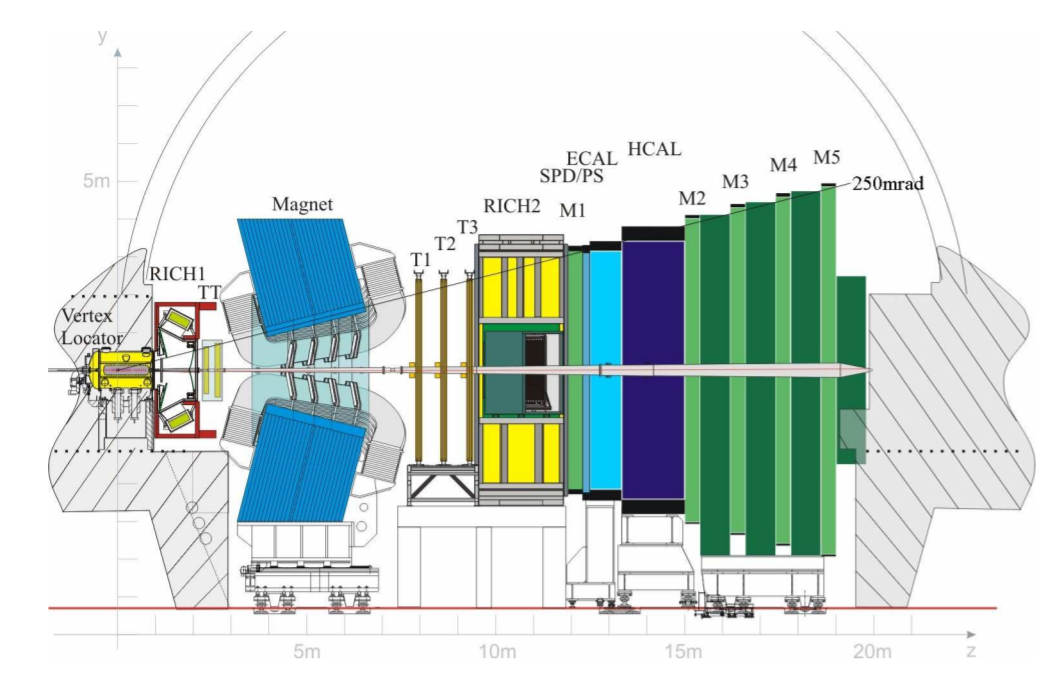
\includegraphics[width=0.9\linewidth]{figures/chapter2/LHCb.png}
  \caption{A cross-section of the LHCb spectrometer in runs 1 and 2, the Velo detector, is visible in the far left of the image.}
  \label{fig:lhcb}
\end{figure}

\section{LHCb subsystems}

This section will briefly discuss LHCb subsystems, apart from the Velo detector, which is discussed in detail in the next section.
The order of the presentation of the subsystems follows their position along the beam axis (see Fig. \ref{fig:lhcb}), that is also the z-axis of the LHCb global coordinate system.

\subsection{Rich}
Ring Imaging Cherenkov detectors (RICH-1 and RICH-2) uses the Cherenkov effect to identify charged hadrons.
RICH-1 is closer to the interaction point and detects lower momentum particles ($~1-60GeV/c$). RICH-2 is downstream after the magnet and is optimised to detect hadrons with momenta in the range ($~15-100GeV/c$)
Both detectors are using different radiation mediums for Cherenkov effect. RICH-1 is using aerogel and $C_{4}F_{10}$, RICH-2 is using $CF_{4}$.
The different media and different Cherenkov angles produced by the particles, with a combination of the momentum information of particle, allow to distinguish protons, kaons and pions with high precision.


\begin{figure}
  \centering
  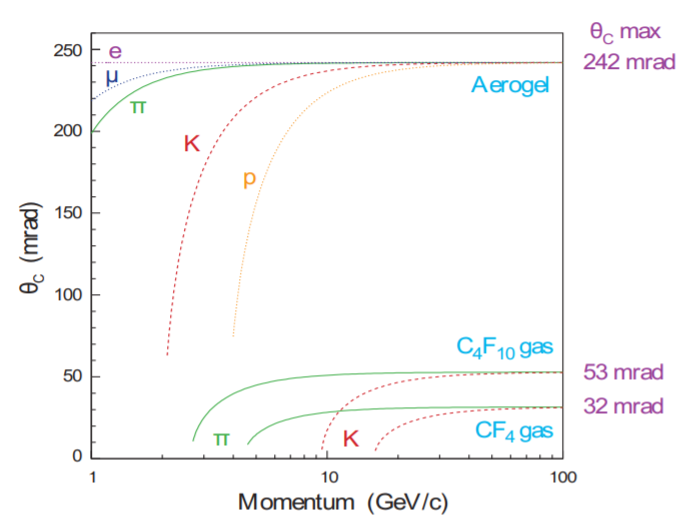
\includegraphics[width=0.55\linewidth]{figures/chapter2/cherenkov_mediums.png}
  \caption{Different media used in RICH with different Cherenkov angles versus their momentum, with different particles.}
  \label{fig:cherenkov_media}
\end{figure}

\subsection{Trackers}
Apart from the Velo, the tracking subsystem can be divided into three parts: Trigger Tracker (TT), Inner Tracker (IT) and Outer Tracker (OT) \cite{Barbosa-Marinho:582793, Collaboration:1647400}.
The IT and TT make up a Silicon Tracker (ST), which utilises the silicon microstrip technology, similar to Velo.
The TT is located upstream and is a 150 cm wide and 130 cm high planar detector between the magnet and the RICH-1 (see Fig. \ref{fig:st_ot}), and the IT station covers a 120 cm wide and 40 high cross-shaped region in the centre of the OT.
The ST was designed with a single hit resolution of 50 $\mu m$
Each of the trackers has four layers which utilise ``xuvx'' topology (two inner layers are rotated by a stereo angle of $+/-5^{o}$, as presented in Fig. \ref{fig:TT}).
The OT is a detector comprising of gas-tight straw-tube modules, with the 4.9 mm inner diameter of the straws. The inner gas is a mixture of Argon (70\%) and $CO_{2}$ (30\%). The gas composition was chosen to guarantee fast drift time  (less than 50 ns) and good drift-coordinate resolution (200 $\mu m$).
It comprises three stations, marked as T1, T2, and T3 in Fig. \ref{fig:lhcb}.
Each of the stations consists of 4 layers employing a similar topology $x-u-v-x$ of the straws, with $+/-5^{o}$ stereo angle.
All of the stations consist of two retractable halves, but unlike the Velo, they are only retracted when servicing.
These halves consist of short modules (S-type) and long modules (F-type).
The F-type modules contain a staggered layout of 256 straws, and the S-type modules containing 128 single straws.
The S-type modules are located closest to the beam and are half of the length of the F-type to compensate for the space for the beam.
In total, there are 168 F-type and 96 S-type modules,

\begin{figure}[H]
\begin{subfigure}[b]{0.45\textwidth}
  \centering
  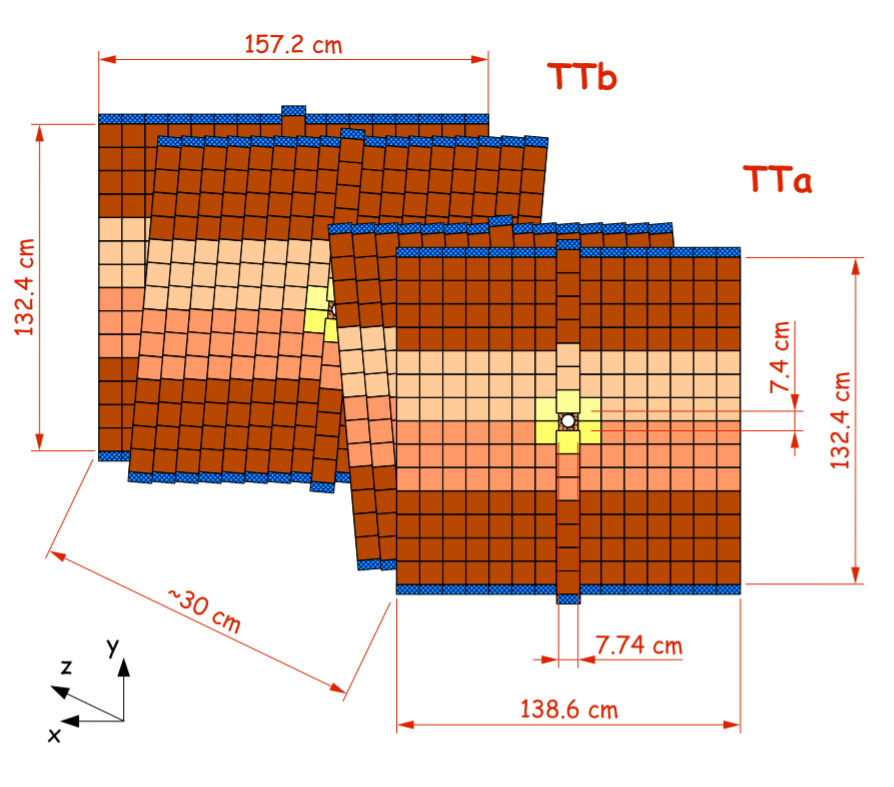
\includegraphics[width=\linewidth]{figures/chapter2/TT.png}
  \caption{TT stations positioning \cite{Knecht:1214889}}
  \label{fig:TT}
  \end{subfigure}
\begin{subfigure}[b]{0.45\textwidth}
  \centering
  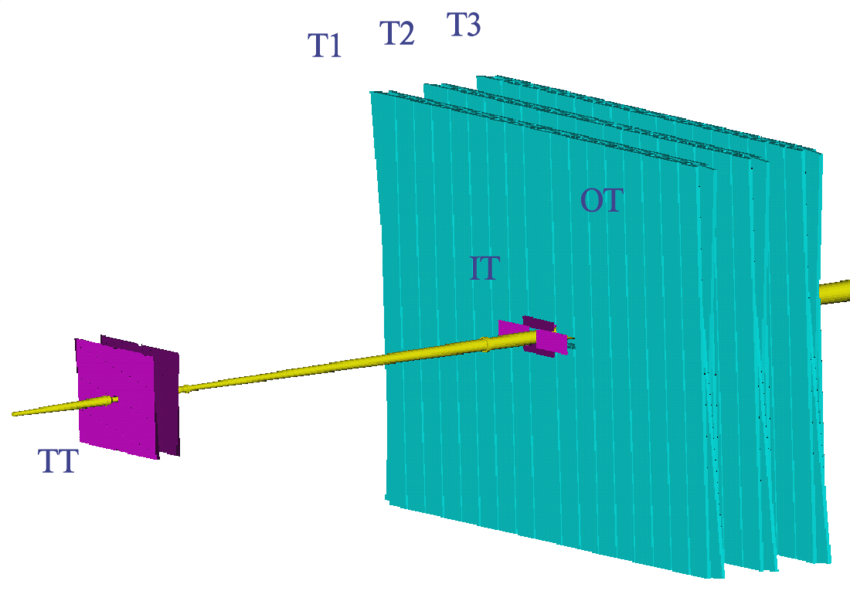
\includegraphics[width=\linewidth]{figures/chapter2/The-main-tracking-system-of-LHCb-TT-IT-and-OT.png}
  \caption{Silicon tracker and outer tracker \cite{alignment-overview}}
  \label{fig:st_ot}
  \end{subfigure}
\end{figure}

\subsection{Magnet}

Next to the TT stations, depicted in blue at Fig. \ref{fig:lhcb}, there is a massive warm, dipole magnet of 1600 tonnes of weight between the tracking stations. Its purpose is to bend the charged particles' trajectory to determine their charge and momentum.
High performance LHCb tracking system requires that the field generated by the magnet has to be carefully mapped with the precision better than $0.1$ \textperthousand.


\subsection{Calorimeters}
The calorimeter system at LHCb consists of three components: PS/SPD (preshower detector/scintillator pad detector), ECAL (electromagnetic calorimeter) and HCAL (hadronic calorimeter).
There are two common types of showers in the calorimetry world: electromagnetic showers and hadronic showers.
When the electron or positron enters scintillating active material, it emits a photon.
A photon, in turn, dissociates to an electron-positron pair, which creates a positive feedback loop that creates more and more particles.
This is known as an electromagnetic particle shower and is depicted in Fig \ref{fig:em_shower}.

\begin{figure}[ht]
  \centering
  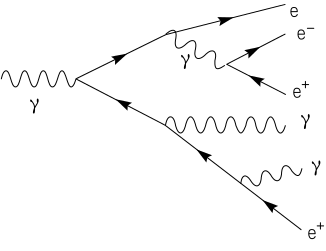
\includegraphics[width=0.35\linewidth]{figures/chapter2/Schematic_of_a_particle_shower.svg.png}
  \caption[something]{Exemplary graph with electromagnetic particle shower\footnotemark. }

  \label{fig:em_shower}
\end{figure}

\footnotetext{ Image source: \url{https://commons.wikimedia.org/wiki/File:Schematic_of_a_particle_shower.svg} }

The hadronic particle shower is more complicated and involves interaction via the strong force.
The electromagnetic calorimeter was created for the purpose of capturing electromagnetic showers.
The rejection of the high-energy charged pion showers in the ECAL requires a PS detector placed in front of the ECAL.
Furthermore, neutral pion showers also must be rejected. For this reason, the SPD detector was positioned in front of the PS detector, separated by a lead converter.

The electromagnetic shower is induced more easily and is shorter than the hadronic one.
The HCAL is much denser and bigger to allow for complete deposition of the energy of the hadronic shower.

\subsection{Muon station}

\begin{figure}
  \centering
  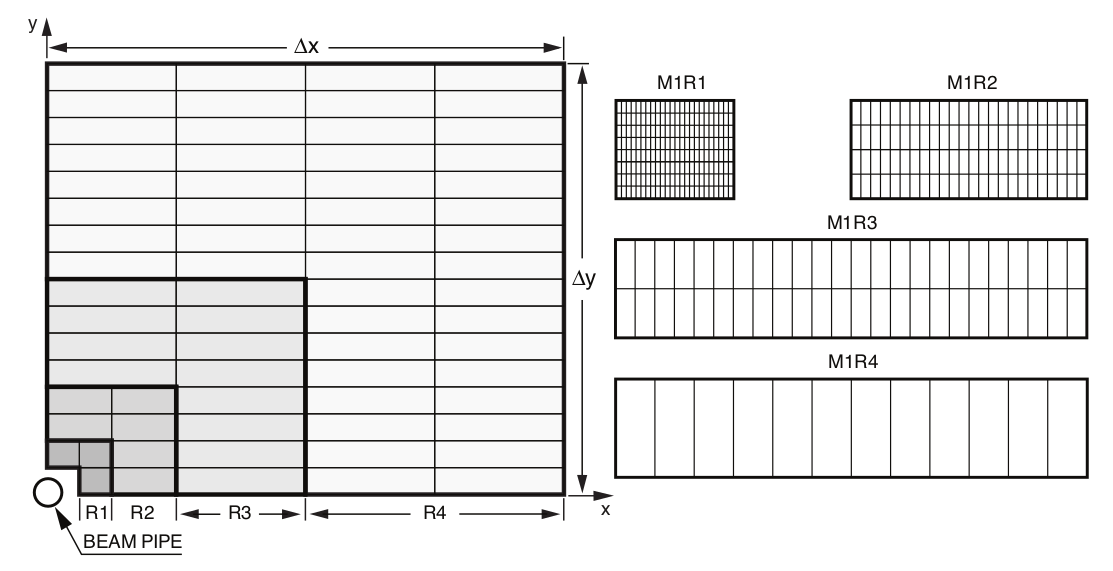
\includegraphics[width=0.9\linewidth]{figures/chapter2/muon_system_partition.png}
  \caption[somethingelse]{Left: front view of a quater part of the muon station, each part reperesents a single region (R1, R2, R3, R4). Right: Division of the each of four region chambers into logical pads.} 

  \label{fig:muon_partition}
\end{figure}

The muons are about 200 times heavier particles than the electrons and exhibit much less energy deposition in matter. In a typical case muon detectors are positioned at the outermost part of the setup (this is the case for LHCb spectrometer). Muons, thanks to their properties constitute a very convenient objects to trigger on. 

In LHCb, the muons system consists of five stations (M1-M5). It is a gas detector consisting of a total of 1380 chambers.
The stations M2-M5 are positioned downstream, and between each station, there is an iron absorber 80 cm thick.
All of the stations utilise MWPC (multi-wire proportional chambers) technology, except for the inner region of the M1 station, which uses triple-GEM (gas electron multiplier) detector chambers.
All stations are divided into four regions, R1, R2, R3, and R4, corresponding with the 1:2:4:8 ratio of length from the beam (as seen at \ref{fig:muon_partition}).
The inner space of MWPC is filled with a mixture of $Ar/CO_{2} /CF_{4}$ (40 : 55 : 5), and contains a wire plane of 2 mm spacing, symmetrically placed in a 5mm gap. This allows for 5ns time resolution.
Each chamber consists of four gaps with wires.


\section{Velo}

The Velo detector (Vertex Locator) is the heart of the LHCb spectrometer.
Its main goal is to record the charged particles' trajectory and reconstruct the collision point with extreme precision. As mentioned in the previous section, the composition of the LHCb spectrometer is changed in upcoming Run 3. The Velo detector is (as of the time of writing) being upgraded from a silicon micro-strip detector to a silicon pixel matrix detector. Because of the possible confusion I assumed the following naming convention throughout my Thesis. I will refer to the upgraded detector as ``VeloPix'', and to the detector used in Run 1 and Run 2 as  ``Velo Strip'' or simply ``Velo''. The readout chip is called VeloPix ASIC or VeloPix chip.

\subsection{Strip Velo in Run 1 and 2}

The Velo in the Run 1 and 2 consists of 42 modules.
Each of the modules is comprised of 2 sensors: $R$ and $\phi$-type.
Each sensor side is a silicone microstrip sensor.
The individual sides correspond to different polar coordinates, as depicted at Fig. \ref{fig:velo_routing}.
Each sensor had 2048 silicon strips (physical channels).
In total, it gives more than 170 000 strips in the entire Velo detector.


\begin{figure}[H]
  \centering
\begin{subfigure}[t]{0.7\textwidth}
  \centering
  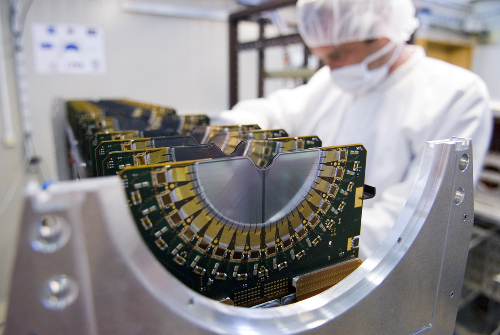
\includegraphics[width=\linewidth]{figures/chapter2/velo_assembly.jpg}
  \caption{Strip Velo during assembly\footnotemark. }
  \label{fig:velo_assembly}
  \end{subfigure}
\begin{subfigure}[t]{0.7\textwidth}
  \centering
  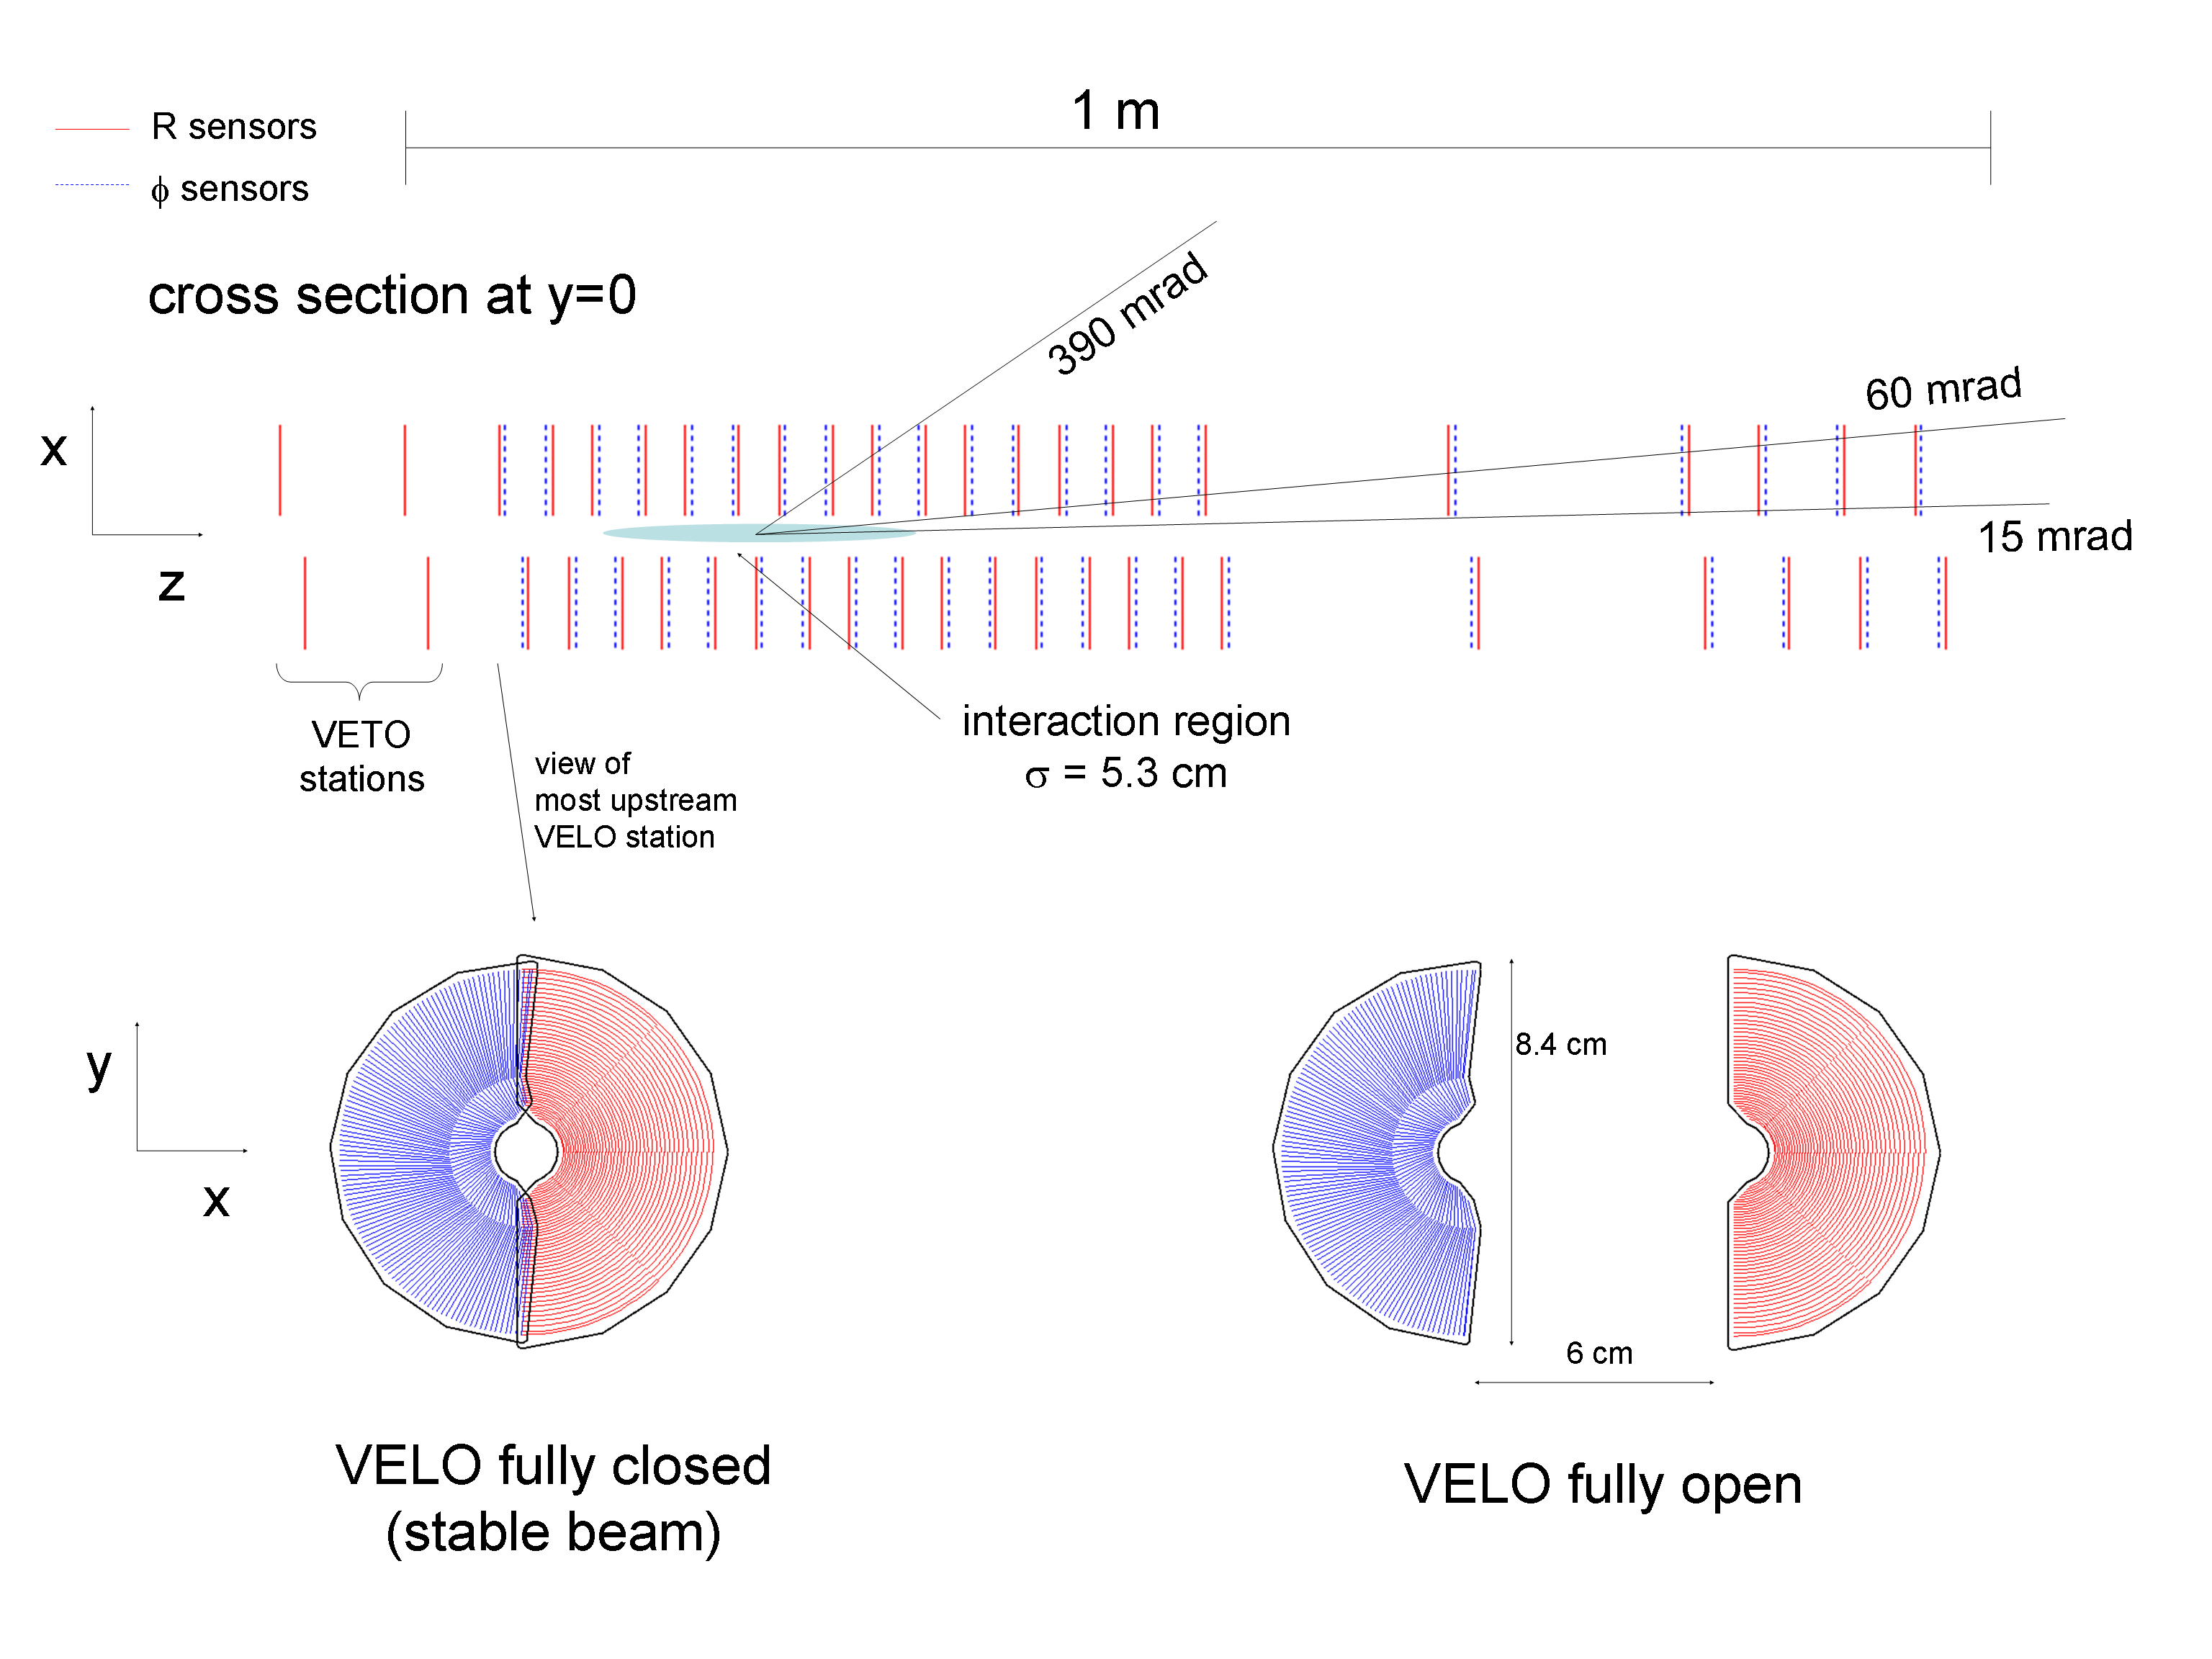
\includegraphics[width=\linewidth]{figures/chapter2/veloOverview.png}
  \caption[overview]{Overview diagram showing the spacing of modules along Z and positions open and closed.}
  \label{fig:velo_overview}
  \end{subfigure}
\end{figure}

\footnotetext{ Image source: \url{ https://lbtwiki.cern.ch/bin/view/VELO/VELOConferencePlots} }

Velo modules are mounted on two retractable halves, which enclose the beam. The movable construction is necessary to protect the LHC beam during the injection stage, before the stable beam condition is achieved.
One of the halves is visible in the Fig. \ref{fig:velo_assembly}.
The alignment of the modules on the halves is staggered as depicted in Fig. \ref{fig:velo_overview}.
Additionally to 42 two-sided modules, four VETO stations are positioned on the other side of the interaction point, consisting of only R-type sensors. The VETO stations proved very useful to provide information to the trigger system and measure the rapidity gap.

The Velo detector (both Velo Strip and VeloPix) is enclosed in its own secondary vacuum tank, which is separated from the primary beam vacuum.
The geometry of the inner gap of sensors is 8mm in radius, and the outer radius of the sensor is about 42 mm.
When the stable proton beam is decalred, the halves of the detector are being retracted (so called closing procedure), which requires the precise position of the collision point to be calculated.
After that, the halves of the Velo detector are moved closer gradually towards the beams using stepper
motors. Sensors get as close as 7 mm to the interacting beams. \cite{Aaij:1707015}.
The sensors themselves are created using oxygenated $n^{+}$-on-$n$ technology, consisting of $n^{+}$-type implant on a $n$-type bulk with a back-plane of $p^{+}$-type implant.
With an exception for two most upstream modules that where produced using the $n^{+}$-on-$p$ silicon type.

The sensors are 300 $\mu m$ thick, and their spatial separation (pitch) varied as a function of radius \cite{Barbosa-Marinho:504321} as depicted on the \ref{fig:velo_pitch}. The way that physical sensor strips were arranged, with their routing lines, influences the ordering of the data and the calibration procedure.

\begin{figure}
  \centering
  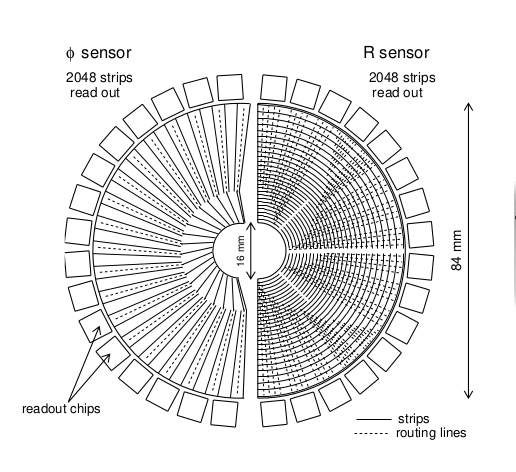
\includegraphics[width=0.7\linewidth]{figures/chapter2/velo_module_routing.png}
  \caption{A depiction of Velo sensors and their routing lines.
    This is just the schematic representation as it does not reflect the actual number of strips and routing lines.
    The $\Phi$-type sensors' outermost strips are directly connected to the readout chips without a need for long routing lines, but the innermost part has routing lanes lying parallel to the outermost strips.
    The $R$-type sensor routing is divided into sections of routes with different lengths.
    In reality, both sensors are divided into 512 long sections of repeated routing lines lengths.
  }
  \label{fig:velo_routing}
\end{figure}

\begin{figure}
  \centering
  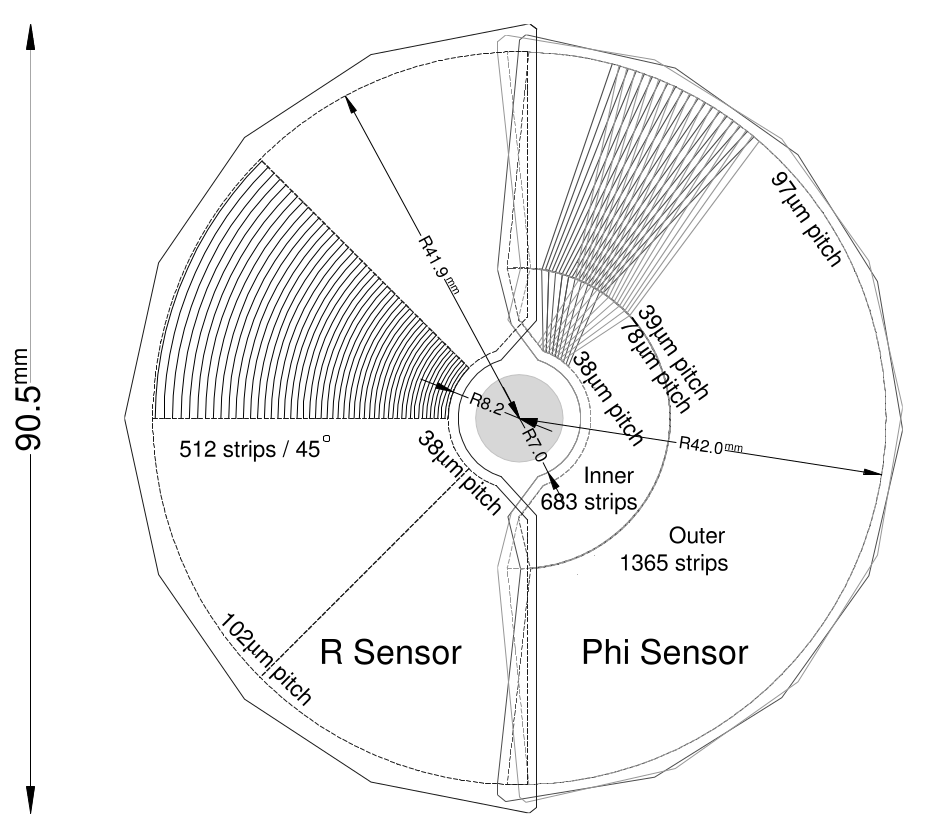
\includegraphics[width=0.7\linewidth]{figures/chapter2/velo_module_pitch.png}
  \caption{ A detailed view of the Velo sensors with their according pitch. The R sensor's pitch starts at 38$\mu m$ and ends on 102$\mu m$. The $\Phi$-type sensors' pitch modulation is divided in two. The most inner 683 strips have from 38 $\mu m$ to 78 $\mu m$ pitch, and the outer rest has a pitch ranging from 39 $\mu m$ to 97 $\mu m$. }
  \label{fig:velo_pitch}
\end{figure}


As seen in the Fig. \ref{fig:velo_routing}, the ordering of the R-type sensor routing lines is divided into four sectors and varies in the distance of the strip from the centre (proton beam). What is not visible in the Fig. \ref{fig:velo_routing} (because of the simplification of the plot) is that the $\Phi$-type sensor is also divided into two parts (as seen in the \ref{fig:velo_pitch}).

The silicon strips are connected to the Beetle front-end ASICs that are mounted on the Velo module board.
Each Beetle chip has 128 indivudually instrumented readout channels. In the case of Velo the signals read from the detector are only conditioned by the analogue part of the chip and send via 60 m long copper cables for digital processing to the electronics Tell1 boards. 
The strips are sampled with 40 MHz frequency and internally queued \cite{Löchner:1000429} in an analogue pipeline.
The analogue data are brought off-chip at 1.1 MHz, with 32 channels multiplexed over four lines.

As mentioned above, the data readout from the Beetle chips was passed to Tell1 boards.
The Tell1 boards have been standardised for the entirety of the LHCb detector.
They accept either optical or analogue receiving cards.
The information was then processed on the on-board FPGAs with custom processing algorithms.
From the Tell1 electronics, the data was transferred to higher-level systems like ECS (Experimental Control System) and triggers.

\subsubsection{Calibration procedure for Velo}
\label{chap2:calibration}
% http://cds.cern.ch/record/1074928/files/lhcb-2007-151.pdf
% https://inspirehep.net/files/83cebd5d85f3494474861bf522e0bbb9
In the absence of proton-proton collisions, the signal observed on each Velo readout channel is approximately normally distributed.
In the first place, the calibration procedure aims to shift the central value of each of these distributions to zero (so called base-line correction).
As shown in the top plot in Fig. \ref{plot:postcal} this offset (also called the pedestal) is, in general, different for each individual channel and needs to be evaluated by a dedicated algorithm using RAW Non-Zero Suppressed Velo data taken without colliding beams.
The equalised Non-Zero Suppressed data are shown at the bottom of Fig. \ref{plot:postcal}.
After the offset correction is applied (called the pedestal $P$ subtraction,\cite{Aaij:1707015}) the noise can be estimated in each channel as the width of the signal distribution.

\begin{figure}
    \centering
    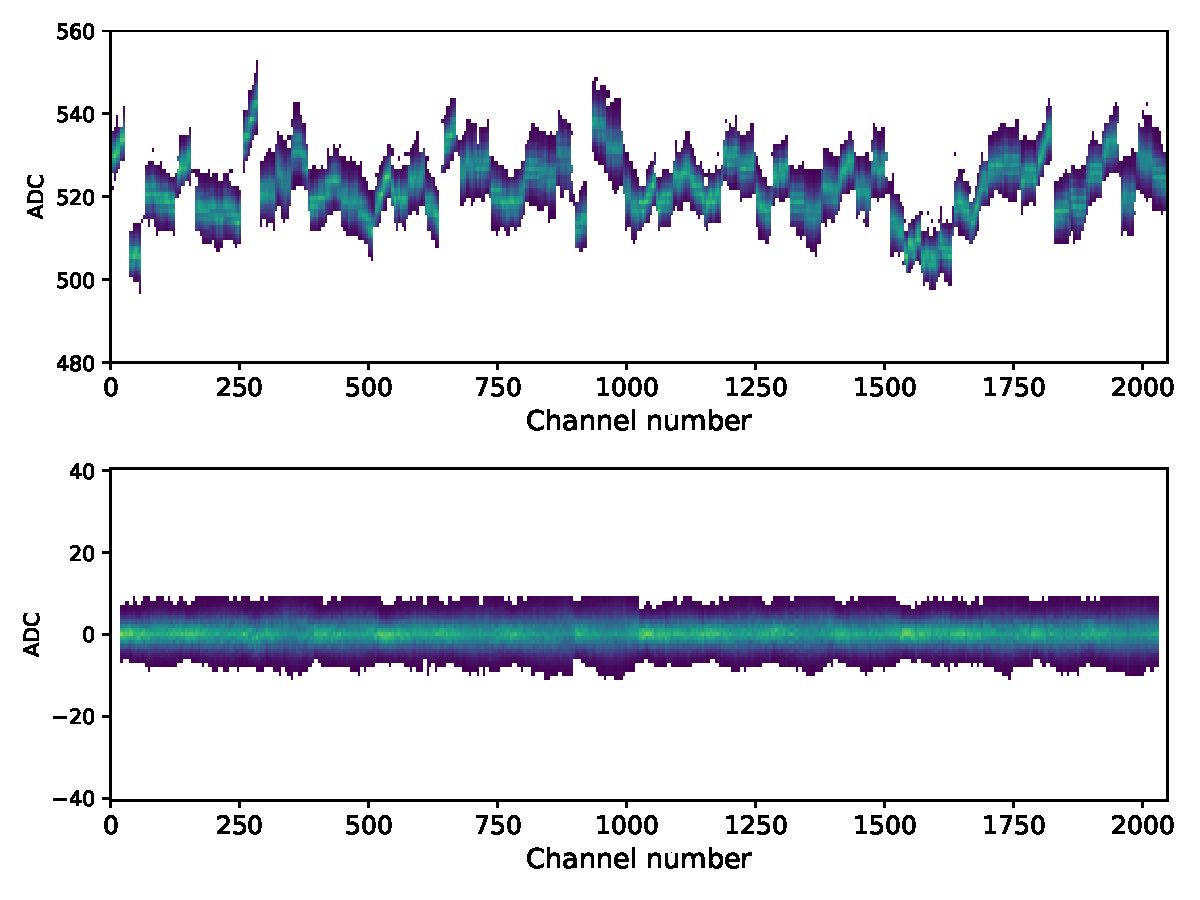
\includegraphics[width=0.7\linewidth]{figures/chapter2/pre_post_cali.pdf}
    \caption[thing]{Typical RAW Non-Zero Suppressed Velo data before (top) and after the digital processing (bottom). The response of each channel was equalised, and a common flat baseline centred on 0 ADC\footnotemark achieved. The spread of the data points about the baseline is attributed to the total noise present in the system.}
    \label{plot:postcal}
\end{figure}

\footnotetext{Where ADC is Analogue to Digital Count that represents the amplitude of the signal after the digitisation.}

The noise evaluated during the calibration procedure is vital for the hit detection and cluster reconstruction algorithm since it is used to suppress the channels without high ADC counts (Zero Suppression procedure). Here, there is an assumption of the correlation between charged particles passing through sensors and depositing the energy in their active volume and the signal amplitude measured on each readout strip.
The performance of the cluster reconstruction  algorithm is of critical importance for the Velo data quality.
The algorithm is comprised of two stages hit detection and cluster building.
The former step relied on so-called high thresholds evaluated for each channel using the measured noise.
For each channel, the high threshold, $H_t$, was set to be five times higher than the noise measured on this channel.
Taking into account the approximate Gaussian nature of the signal distribution without particle hits, it corresponds to the probability of accepting a noise signal as a real hit at the level of $10^{-7}$.
The cluster building step used the selected channels that passed the hit detection algorithm as seeds.
Clusters were formed by searching for the secondary signal channels using so-called, low hit thresholds.
Up to four channels were used to form a single cluster.

In general, the clustering algorithm works as follows\cite{Parkes:1074928}:
\begin{enumerate}
  \item If the measured signal exceeded the high threshold $H_{t}$ on strip $S_{n}$, then the channel was tagged as the cluster seed.
  \item In the next step, the signal measured on the adjacent strips, with respect to a seeding strip, were compared to the low thresholds. All strips that passed the low threshold cuts were tagged, along with the seeding strip, as a cluster candidate
  \item In the last step, a cluster (hit) was built. A global cut on the cluster size was set to four strips. In case when a cluster candidate is comprised of more strips, the algorithm creates multiple adjacent clusters. Finally, the local position of each created cluster was evaluated using a centre of gravity formula.
\end{enumerate}

A visualisation of the algorithm can be found in the Fig. \ref{plot:velo_clustering}.

\begin{figure}
    \centering
    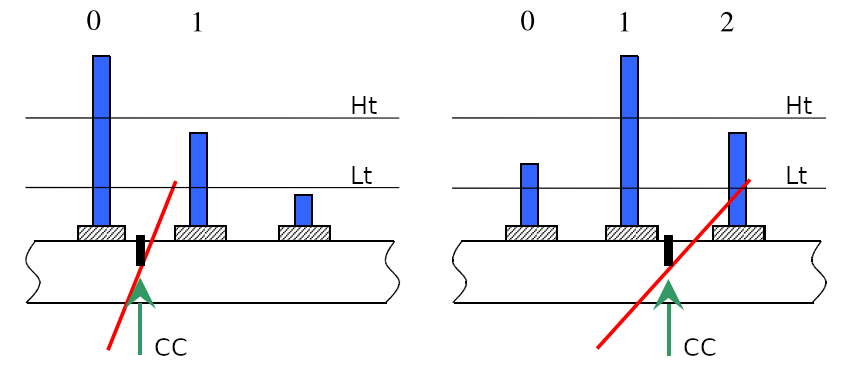
\includegraphics[width=0.7\linewidth]{figures/chapter2/clustering_algorithm_velo.png}
    \caption{Visualisation of the clustering algorithm. Two examples of Velo clusters are shown schematically. Blue rectangles depict the charges collected on the strips. Black lines represent high threshold $H_{t}$ and low threshold $L_{t}$ cuts, the reconstructed cluster centre (CC) is indicated by arrows and the particle trajectory is given by the red sloping lines.}
    \label{plot:velo_clustering}
\end{figure}

\subsubsection{Header Cross-Talk}
\label{chap2:headercrosstalk}

The Beetle chips in Velo are connected to 128 physical strips and send data on four analogue links, with 32 channels of analogue data.
There is a pseudo-binary information header preceding the analogue data.
This information consists of four bits and encodes the status of the front-end chips and the pipeline column number.
Unfortunately, this caused a problem in the data transfer, and the four preceding bits induced an additional noise in the first upcoming data channel.
In total, this contributed to the increased noise in 64 channels in Velo sensor.
This effect is known as header cross-talk\cite{Szumlak:1177860}. The initial commissioning studies, performed before Run 1, showed that this can produce a significant stream of fake clusters increasing the volume of the Velo data transmitted to the high-level trigger. A dedicated correction algorithm has been developed in order to alliviate the problem.

\subsubsection{Voltage and luminosity}
\label{chap2:lumivolt}

Each of the strips in Velo is, in essence, a semiconductor diode. It is an $n^{+}$-type implant in an n-type bulk with a back p-type implant\cite{Akiba:2633496}.
The physical process of exciting the matter electromagnetically inside the sensor bulk creates a cloud of electrons and holes.
For the charge to be able to cross the depletion region, there needs to be additional bias voltage applied.
This is also a way of mitigating the radiation damage, as the multiple negative factors disrupt the flow of the generated charge.
The Fig. \ref{fig:radiation_damage}, shows that the bias voltage necessary for the optimal operation of the Velo detector has been steadily growing along with the delivered integrated luminosity.

\begin{figure}[H]
  \centering
\begin{subfigure}[t]{0.654\textwidth}
  \centering
  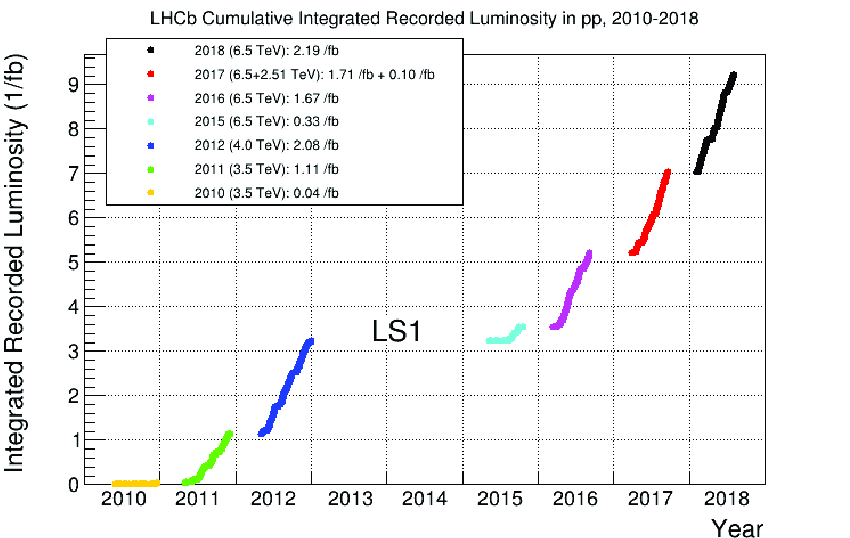
\includegraphics[width=\linewidth]{figures/chapter2/LHCb-Cumulative-Integrated-Recorded-Luminosity-in-pp-2010-2018.png}
  \caption{Integrated luminosity for the years 2010-2018 \cite{Kurbatov}.}
  \label{fig:velo_lumi}
  \end{subfigure}
\begin{subfigure}[t]{0.65\textwidth}
  \centering
  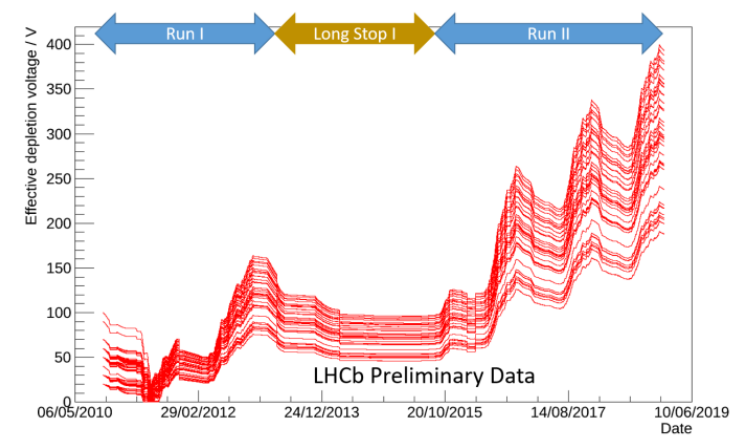
\includegraphics[width=\linewidth]{figures/chapter2/velo_strip_voltage.png}
  \caption[stripvo]{Projected Velo bias voltage.}
  \label{fig:velo_voltage}
  \end{subfigure}
  \caption[]{Radiation damage effects on the LHCb Velo.}
  \label{fig:radiation_damage}
\end{figure}


\subsection{Velopix}

The Large Hadron Collider and its detectors were planned to be incrementally
improved over time. In LHC Run 3, there will be a significant increase
in the instantaneous luminosity, and the Velo must adapt to that change. For this purpose the Velo group proposed to change the sensor technology from planar strip sensors to pixel ones
read-out by the VeloPix ASIC that was adapted from the TimePix chip, which belongs to MediPix family of sensors.

Some of the requirements for the upgraded detector include:
\begin{itemize}
\item \textbf{Increased rate of data} output to 40 MHz with hits/event $≈ 5.2cm^{-2} \times R^{−1.9}$ (R is radius in $cm$).
This means that the VeloPix ASICs must be able to output up to 15.1 GB/s. The peak total data rate of upgraded Velo can reach up to 2.85 Tbit/s.
\item \textbf{Irradiation} the upgraded detector is predicted to experience an accumulated the flux of fast hadrons
$∼ 8 \times 10^{15}n_{eq} /cm^{2}$, and when this is reached, it is expected that the bias voltage and the current necessary for operating the sensors at the pixel closest to the beam will be $1000V$ and $200 \mu A/cm^{2}$ at -20C.
Such a high dose of radiation and high currents will make a significant obstacle in protecting the sensor from thermal runaway.
\end{itemize}


\begin{figure}
  \centering
  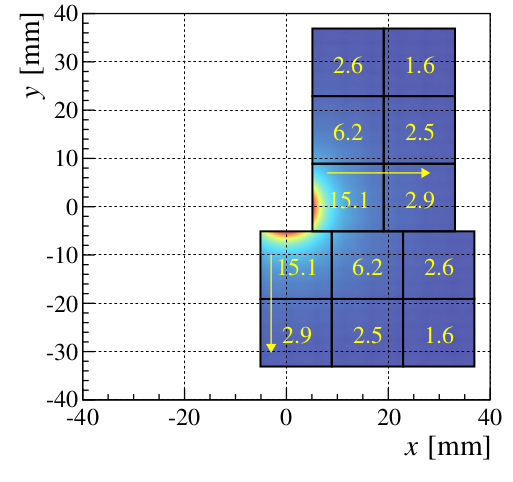
\includegraphics[width=0.4\linewidth]{figures/chapter2/data_rate.png}
  \caption{The projected data rate for each ASIC in Velo module (in Gbit/s).}
  \label{fig:velopix_datarate}
\end{figure}
\begin{figure}
  \centering
  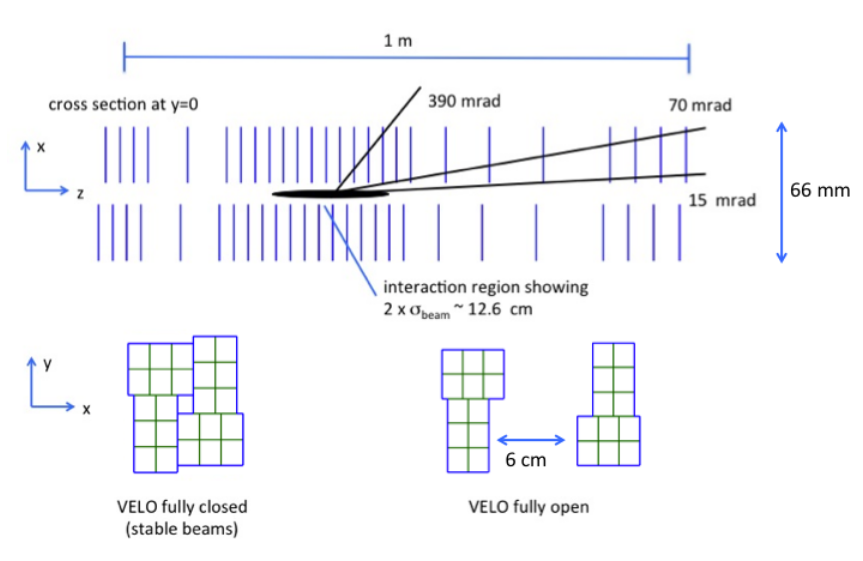
\includegraphics[width=0.7\linewidth]{figures/chapter2/velopix_layout.png}
  \caption{  }
  \label{fig:velopix_layout}
\end{figure}

The new upgraded Velo detector that will collect data during Run 3 and Run 4 has a modular design, similar to the previous strip device. Each module contains 4 sensors, each sensor is readout by
3 VeloPix ASICs. VeloPix chips are rectangular in shape and can readout matrices of 255x255 pixels.
New Velo sensors feature square $55 x 55 \mu m^{2}$ pixels that provides excellent spatial resolution. 
There are 52 modules arranged along the z-axis (i.e., along the LHC beam). It is worth noticing that significant portion of the Velo strip detector's infrastructure remained, for instance the secondary vacuum tank.
A simplified visualisation of the Velo modules z-positions and the pixel sensors geometry is shown in Fig. \ref{fig:velopix_layout}.

In order to process the data more effectively and save the transmission bandwidth individual pixels are grouped on the logical level in, so called, super-pixels.
Super-pixels consist of eight pixels arranged as 2 by 4 matrices.
Sending data using the super-pixels instead of pixels allows for a reduction of the total required bandwidth by about 30\% \cite{Collaboration:1624070}.
When there is a hit in the super-pixel, a 9-bit timestamp is created and stored.
Each super-pixel can store up to two timestamps.
Readout from the super-pixels is done via a 23-bit bus running at 13.3 MHz.
This means that there is a data transfer only when there is a hit information. In other words, the new VeloPix detector is a trigger-less system.

\subsubsection{Velopix masking}
\label{chap2:velopix_calibration}

A critical functionality of both vertex systems is a possibility to deactivate a problematic readout channels, also called "bad" channels. Typical reasons for deactivation can be related with sensor issues (for instance physical damage), problems with bonds (broken bond or partially connected bond) or readout lines. The best strategy to identify bad channels is to measure and trend noise.
The procedure of collecting the noise data (without proton-proton collisions), identifying problematic channels and then disabling them is called masking.

During the Run 1 and Run 2 operation a significant experience was gained related to this important issue. There was a fraction of bad channels that were considered "fixed" and they do not changed over time, however, a majority of them did not show permanent problems and evolved in time. 
Quick tagging of bad channels was essential for keeping the high data quality. 
For instance, a large number of noisy channels will create a stress in trigger readout system by producing spurious fake hits. This may degrade the tracking and increase processing time due to larger number of hits. 

In case of the pixel detector, that operates in trigger-less mode, large number of unmasked noisy channels can completely saturate the readout lines, since the fake hits will be sent constantly (in case of the strip detector it would be just one fake cluster per one trigger). Evaluation of the set of pixels to be masked will be performed during the, so called, equalisation that is the core of the VeloPix calibration procedure. The number and distribution of the masked channels must be carefully study and monitor during the data taking period. A short description of the equalisation is given below.





\begin{figure}
    \centering
    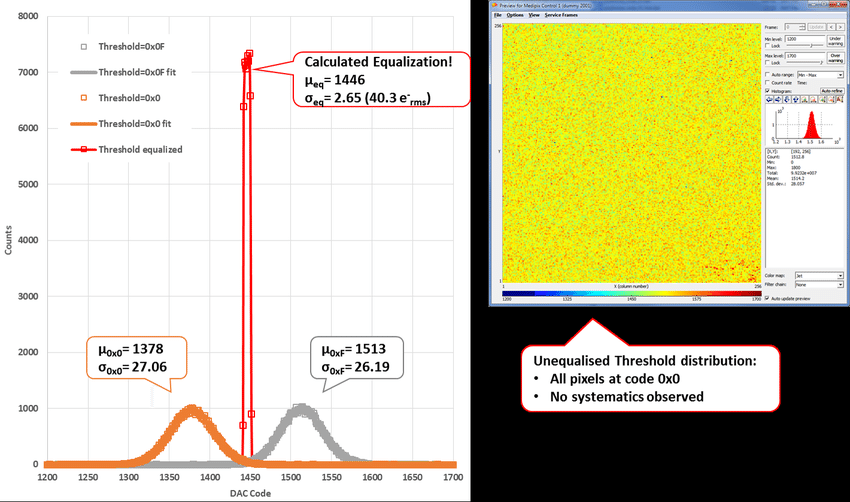
\includegraphics[width=0.7\linewidth]{figures/chapter2/Threshold-spread-in-the-pixel-matrix.png}
    \caption{Exemplary threshold spread of the pixel matrix.}
    \label{plot:velopix_thresholding}
\end{figure}

% https://lbtwiki.cern.ch/bin/view/VELO/VeloUpgradePresentationMaterial
% @TODO add images

% https://www.researchgate.net/publication/312869714_The_VeloPix_ASIC // \cite{poikela}
% https://www.researchgate.net/publication/224577931_Optimization_of_Medipix-2_Threshold_Masks_for_Spectroscopic_X-Ray_Imaging#pf5
% http://cds.cern.ch/record/2636158/files/VeloPix%20Data%20Visualisation%20and%20Read-out%20Control.pdf
% https://cds.cern.ch/record/2723996/files/2006.09559.pdf
% https://www.researchgate.net/publication/291436661_Equalization_method_for_Medipix3RX
\subsubsection{Velopix Calibration}
Similarly to strip Velo, VeloPix will collect the noise calibration data \cite{Kopciewicz:2723996}. 
In the case of the VeloPix, each pixel has its own individual voltage threshold. If this
threshold is exceeded by signal induced by a passing charged particle, a hit is registered.
There are two types of values that can be set in a readout chip to define individual thresholds: Global Threshold (GT) and Trim.
The former is evaluated for each sensor matrix (255 x 255 pixels), whilst, the latter are defined per individual pixel,  they are 4-bit numbers (16 different values).
Trim is a readout DAC voltage that is individually added to the signal in the discriminator such that it allows to achieve equal response for each pixel across the whole detector matrix.

For the convenience of the Reader, the automatic procedure that is used to evaluate the GT and Trims is described briefly below. This a counterpart to the Velo Strip calibration and threshold calculation, and might be the key point to transferring many of the solutions described in this thesis to the Run 3. The visualisation of the procedure is shown in Fig. \ref{plot:velopix_thresholding}.

The calibration procedure uses two types of thresholds: a $Trim$, and global threshold $GT$.
The actual threshold (sensitivity) of the pixel is given by the sum of those two.

The first step is to find a distribution of the counts of hits in the lowest trim setting  $Trim_{0}$ and highest trim setting $Trim_{15}$. This is done by openning the shutter of the sensor for constant of time and counting hits first in lowest trim setting then in the highest. In each of the trim settings the $GT$ is modulated, which leads to creation of two histograms, as visible in Fig. \ref{plot:velopix_thresholding}. $GT$ modulation takes place in predefined range nad step of DAC.
Then, for a low and high bound of all pixels in a sensor, the mean of the distribution $Trim_{0}$ and $Trim_{15}$ are used, to set the $PixelTrim_{0}$ and $PixelTrim_{15}$. Those values are the same for every pixel.

This creates a range for all 16 possibles trims, with the step of the trim being $TrimStep = \frac{PixelTrim_{15}-PixelTrim_{0}}{15}$.

Now to determine which of the trim value should be set for the pixel, we
take advantage of the distribution measured in each of the two scans ($Trim_{0}$ and $Trim_{15}$). Both of those yield noise events distributed normally.
A perfect target of the global threshold $GT_{target} = \frac{TRIM_{0}+TRIM_{15}}{2}$ is set, in the center between two means of the distributions.
Then each of the pixels gain the trim value of $PixelTrim(x,y)$ set as close to
$GT_{target}$, where $PixelTrim(x,y)$ is any trim (integer) from the range $[0..15]$, where $0$ means $PixelTrim_{0}$ and $15$ means $PixelTrim{15}$.
To exclude the noise from the signal coming from the pixels, the
effective global threshold $GT_{effective}$ is set to
$GT_{target} + 1000[electrons]$.
So the actual threshold for the individual pixel
$Th_{x,y} = {PixelTrim(x,y)} + GT_{target} + 1000[electrons]$

% \subsubsection{Calibration example}
% Let's say that we start the scan with global threshold value of $GT = 1100 DAC$, and increase to $1600 DAC$, with a
% step of $1 DAC$.
% %% @TODO ref plot.
% %% @TODO finish example
% For example, if the mean
% from TRIM0 was 1111, and mean from TRIM15 was 1431, this means that the trim
% step is (1411-1111/15) == 20. This means that the TRIM1 is 1131, TRIM2 is 1151 and etc.
